% !TeX root = surprises.tex

\chapter{Trisección de un ángulo}\label{c.trisect}

%%%%%%%%%%%%%%%%%%%%%%%%%%%%%%%%%%%%%%%%%%%%%%%%%%%%%%%%%%%%%%%

Es imposible trisecar un ángulo arbitrario (dividir el ángulo en tres partes iguales) utilizando sólo una regla y un compás. La trisección requiere la construcción de raíces cúbicas, pero una regla y un compás sólo pueden construir longitudes que son expresiones construidas a partir de números enteros, las cuatro operaciones aritméticas y raíces cuadradas. Esto fue demostrado por Pierre Wantzel en 1837. Sin embargo, innumerables aficionados siguen intentando trisecar un ángulo. Sus construcciones son aproximaciones aunque están convencidos de que son correctas. La sección~\ref{s.trisect-approx} presenta dos construcciones de este tipo, desarrolla fórmulas para los ángulos y muestra los errores en las aproximaciones.

Los matemáticos griegos descubrieron que si se permiten otros instrumentos, los ángulos se pueden trisecar. La sección~\ref{s.neusis} explica una construcción de Arquímedes utilizando un instrumento sencillo llamado \emph{neusis} y la sección~\ref{s.neusis-doubling} muestra cómo duplicar el volumen de un cubo utilizando el neusis. La sección~\ref{s.q} presenta una construcción para la trisección de Hipias utilizando un instrumento llamado \emph{cuadratriz}. El resto del capítulo contiene una demostración de la imposibilidad de la trisección de un ángulo. La sección ~\ref{s.trisect-constructible} caracteriza los números construibles, la sección~\ref{s.trisect-poly} relaciona los números construibles con las raíces de los polinomios y la sección~\ref{s.trisect-impossible} utiliza esta teoría para demostrar que la trisección de un ángulo y la duplicación de un cubo son imposibles.

%%%%%%%%%%%%%%%%%%%%%%%%%%%%%%%%%%%%%%%%%%%%%%%%%%%%%%%%

\section{Trisecciones aproximadas}\label{s.trisect-approx}

\subsection{Primera trisección aproximada}\index{Trisection of an angle!approximation}\label{sub.trisect-approx1}

\noindent\textbf{Construcción:}
Sea $\theta=\angle AOB$ un ángulo arbitrario y sin pérdida de generalidad supongamos que $A,B$ están en una circunferencia unitaria cuyo centro es $O$. Bisecamos $\angle AOB$ y sea $C$ la intersección de la bisectriz con la circunferencia unitaria. Sea $D$ el punto medio de la $\overline{OA}$ y sea $T$ el punto medio de la $\overline{DC}$. Denotemos el ángulo $\angle DOT$ por $\phi$ (Fig.~\ref{f.trisect-first-approx-1}).

\begin{figure}[ht]
\begin{center}
\begin{tikzpicture}[scale=.6]
\coordinate (O) at (0,0)
  node[left] {$O$}
  node[above right,xshift=14pt,yshift=16pt] {\sm{\theta/2}}
  node[right,xshift=18pt,yshift=4pt] {\sm{\theta/2}};
\coordinate (A) at (9cm,0);
\node[right] at (A) {$A$};
\coordinate (B) at (60:9);
\node[above] at (B) {$B$};
\draw (A) arc(0:60:9);
\draw (B) -- (O) -- (A);
\coordinate (C) at (30:9);
\node[right] at (C) {$C$};
\draw (O) -- node[above] {$1$} (C);
\coordinate (D) at (4.5,0);
\node[below] at (D) {$D$};
\coordinate (T) at ($(D)!.5!(C)$);
\draw (D) -- node[left] {$a$} (T) -- node[left] {$a$} (C);
\node[right] at (T) {$T$};
\draw (O) -- (T);
\draw (	1,0) arc (0:30:1);
\draw (30:.8) arc (30:60:.8);
\draw (2,0) arc (0:20:2);
\node[above right] at (2.1,0.1) {\sm{\phi}}; 
\draw[<->] (0,-1) -- node[fill=white] {$1/2$} +(4.5,0);
\draw[<->] (4.5,-1) -- node[fill=white] {$1/2$} +(4.5,0);
\end{tikzpicture}
\end{center}
\caption{Primera trisección aproximada (1)}\label{f.trisect-first-approx-1}
\end{figure}

\begin{theorem}
\[\tan\phi =\frac{2\sen(\theta/2)}{1+2\cos(\theta/2)}\,.\]
\end{theorem}

\begin{proof} Figura~\ref{f.trisect-first-approx-2} se extrae de la figura~\ref{f.trisect-first-approx-1} y contiene anotaciones adicionales.

Sea $\overline{CF}$ la perpendicular a $\overline{OA}$ que corta a $\overline{OA}$ en $F$. Dado que $\overline{OC}=1$, $\overline{CF}=\sen(\theta/2)$ y $\overline{OF}=\cos(\theta/2)$. Sea $\overline{TE}$ la perpendicular a $\overline{OA}$ que interseca $\overline{OA}$ en $E$.

$T$ es el punto medio de $\overline{DC}$ por lo que $\overline{DT}=\overline{TC}=a$. Pero $\overline{FT}$ es la mediana de la hipotenusa de un triángulo rectángulo, por lo que $\overline{FT}=a$ y por tanto $\triangle DTF$ es isóceles. Se deduce que $\overline{TE}$ es tanto la mediana como la altitud de $\overline{DF}$. A partir del diagrama es fácil ver que:

\begin{figure}[ht]
\begin{center}
\begin{tikzpicture}[scale=1]
\coordinate (O) at (0,0)
  node[left] {$O$}
  node[right,xshift=24pt,yshift=5pt] {\sm{\theta/2}};
\coordinate (A) at (9cm,0);
\node[right] at (A) {$A$};
\draw (O) -- (A);
\coordinate (C) at (30:9);
\node[right] at (C) {$C$};
\draw (O) -- node[above] {$1$} (C);
\coordinate (D) at (4.5,0);
\node[below] at (D) {$D$};
\coordinate (T) at ($(D)!.5!(C)$);
\draw (D) -- node[left] {$a$} (T) -- node[left] {$a$} (C);
\node[right] at (T) {$T$};
\draw (O) -- (T);
\draw (	1,0) arc (0:30:1);
\draw (2,0) arc (0:20:2);
\node[above right] at (1.9,0.1) {\sm{\phi}}; 

\coordinate (E) at (T |- A);
\draw[thick,dashed] (T) -- node[right] {$h$}
  (E) node[below] {$E$};
\draw[rotate=90] (E) rectangle +(7pt,7pt);

\coordinate (F) at (C |- A);
\draw[thick,dashed] (C) --
  node[right] {$\sen (\theta/2)$} (F) node[below] {$F$};
\draw[rotate=90] (F) rectangle +(7pt,7pt);

\draw[thick,dashed] (T) -- node[right] {$a$} (F);

\draw[<->] ($(O)+(0,-1)$) --
  node[fill=white] {$1/2$} +(4.5,0);
\draw[<->] ($(O)+(0,-1.8)$) --
  node[fill=white] {$\cos (\theta/2)$} ($(F)+(0,-1.8)$);
\draw[<->] ($(D)+(0,-2.6)$) --
  node[fill=white] {$\left(\cos (\theta/2)\!-\! (1/2)\right)$} 
  ($(F)+(0,-2.6)$);
\draw[<->] ($(O)+(0,-3.4)$) --
  node[fill=white] {$(1/2)+(1/2)\left(\cos (\theta/2)\! -\! (1/2)\right)$} 
  ($(E)+(0,-3.4)$);
\end{tikzpicture}
\end{center}
\caption{Primera trisección aproximada (2)}\label{f.trisect-first-approx-2}
\end{figure}

\[
\overline{OE}=\frac{1}{2} + \frac{1}{2}\left(\cos \frac{\theta}{2}-\frac{1}{2}\right)\,.
\]
Calculemos la longitud $2a=\overline{CD}$ utilizando el Teorema de Pitágoras en $\triangle DCF$:
\begin{eqnarray*}
(2a)^2 &=&  \left(\cos \frac{\theta}{2}-\frac{1}{2}\right)^2+\frac{\sen^2\theta}{2}\,.
\end{eqnarray*}
La longitud $h=\overline{TE}$ puede calcularse a partir del Teorema de Pitágoras en $\triangle DTE$:
\begin{eqnarray*}
a^2 &=& h^2 + \left[\frac{1}{2}\left(\cos \frac{\theta}{2}-\frac{1}{2}\right)\right]^2\\
h^2&=&\frac{1}{4}\left(\cos \frac{\theta}{2}-\frac{1}{2}\right)\sen^2+\frac{1}{4}\sen^2\frac{\theta}{2}-\left[\frac{1}{2}\left(\cos \frac{\theta}{2}-\frac{1}{2}\right)\right]^2=
\frac{1}{4}\sen^2\frac{\theta}{2}\\
h&=&\frac{1}{2}\sen\frac{\theta}{2}\\
\tan\phi &=&\frac{h}{\overline{OE}}=\displaystyle\frac{\displaystyle\frac{1}{2}\sen\frac{\theta}{2}}{\displaystyle\frac{1}{2}+\frac{1}{2}\left(\cos \frac{\theta}{2}\! -\! \frac{1}{2}\right)}
=\frac{\displaystyle2\sen\frac{\theta}{2}}{\displaystyle 1+2\cos\frac{\theta}{2}}\,.
\end{eqnarray*}                  
\end{proof}

Esta es una aproximación a una trisección $\phi=\theta/3$. Para $\theta=60^\circ$:
\[
\tan^{-1}\left(\frac{2\sen 30^\circ}{1+2\cos 30^\circ}\right)=
\tan^{-1}0.366\approx 20.1^\circ\approx 20^\circ\,.
\]

Tabla~\ref{t.trisect-first} muestra los errores para un rango de ángulos agudos. El error es relativamente pequeño para ángulos pequeños, aumentando a $1\!\!$\% a $85^\circ$.

\begin{table}[t]
\caption{Errores en la primera trisección aproximada}\label{t.trisect-first}
\[
%
\begin{array}{r@{\hspace{5mm}}r@{\hspace{5mm}}r@{\hspace{5mm}}r@{\hspace{5mm}}r}
\hline
\noalign{\smallskip}
\theta ({}^\circ) & \theta/3 ({}^\circ)& \tan^{-1} \phi ({}^\circ) & \mathrm{Error} ({}^\circ) & \mathrm{Error (\%)}\\\hline
\noalign{\smallskip}
  5 &    1.667 &    1.667  &     0.000 &    0.004 \\
 10 &    3.333 &    3.334  &     0.000 &    0.014 \\
 15 &    5.000 &    5.002  &     0.002 &    0.032 \\
 20 &    6.667 &    6.670  &     0.004 &    0.057 \\
 25 &    8.333 &    8.341  &     0.007 &    0.088 \\
 30 &   10.000 &   10.013  &     0.013 &    0.128 \\
 35 &   11.667 &   11.687  &     0.020 &    0.174 \\
 40 &   13.333 &   13.364  &     0.030 &    0.228 \\
 45 &   15.000 &   15.043  &     0.043 &    0.289 \\
 50 &   16.667 &   16.726  &     0.060 &    0.358 \\
 55 &   18.333 &   18.413  &     0.080 &    0.435 \\
 60 &   20.000 &   20.104  &     0.104 &    0.520 \\
 65 &   21.667 &   21.799  &     0.133 &    0.612 \\
 70 &   23.333 &   23.500  &     0.166 &    0.713 \\
 75 &   25.000 &   25.206  &     0.206 &    0.823 \\
 80 &   26.667 &   26.918  &     0.251 &    0.941 \\
 85 &   28.333 &   28.636  &     0.303 &    1.068 \\
 \noalign{\smallskip}
 \hline
 \end{array}
\]
\end{table}

\subsection{Segunda trisección aproximada}\index{Trisection of an angle!approximation}

\noindent\textbf{Construcción:}
Sea $\theta=\angle AOB$ un ángulo arbitrario y sin pérdida de generalidad supongamos que $A,B$ están en una circunferencia unitaria cuyo centro es $O$. Construimos una circunferencia de radio $1/3$ con centro $O$ y que $D$ sea su intersección con $\overline{OA}$. Bisecamos $\angle AOB$ y sea $C$ la intersección de la bisectriz con la circunferencia de radio $1/3$. Construimos la cuerda $\overline{CD}$ y las cuerdas $\overline{AE}=\overline{ET}=\overline{CD}$. Como cuerdas iguales subtienden ángulos centrales iguales $\angle TOE=\angle EOA=\phi$ (Fig.~\ref{f.trisect-second-approx}).

\begin{figure}[ht]
\begin{center}
\begin{tikzpicture}[scale=.75]
\coordinate (O) at (0,0)
  node[left] {$O$}
  node[above right,xshift=10pt,yshift=12pt] {\sm{\theta/2}};

\coordinate (A) at (9cm,0);
\node[right] at (A) {$A$};
\coordinate (B) at (60:9);
\node[above] at (B) {$B$};
\draw (A) arc(0:60:9);
\draw (B) -- (O) -- (A);
\coordinate (D) at (3,0);
\node[below] at (D) {$D$};
\draw[name path=third] (D) arc(0:60:3);
\coordinate (C) at (30:3);
\node[right] at (C) {$C$};
\draw (O) -- node[above,near end] {\sm{1/3}} (C);
\draw[thick] (D) -- (C);
\coordinate (E) at (10:9);
\node[right] at (E) {$E$};
\draw[thick] (A) -- node[right] {\sm{1/3}} (E);
\coordinate (T) at (20:9);
\node[right] at (T) {$T$};
\draw[thick] (E) -- node[right] {\sm{1/3}} (T);
\draw (O) -- node[above,near end] {$1$} (T);

\draw (	1,0) arc (0:30:1);
\draw (30:.8) arc (30:60:.8);
\draw (4,0) arc (0:20:4);
\node at (4.2,0.35) {$\phi$}; 
\node at (4.1,1.1) {$\phi$}; 

\draw[dashed] (O) --
  node[fill=white,inner sep=0pt,very near start,
       xshift=7pt,yshift=1pt] {\sm{\theta/2}} 
  node[fill=white,near end] {$1$} (E);

\draw[<->] (3,-.8) -- node[fill=white] {$2/3$} +(6,0);
\draw[<->] (0,-.8) -- node[fill=white] {$1/3$} +(3,0);
\end{tikzpicture}
\end{center}
\caption{Segunda trisección aproximada}
\label{f.trisect-second-approx}
\end{figure}

\begin{theorem}
\[
\cos\phi=1 - \frac{1}{9}(1-\cos(\theta/2))=1 - \frac{2}{9}\sen^2(\theta/4)\,.
\]
\end{theorem}
\begin{proof} Por la Ley de los Cosenos en $\triangle DOC$:
\[
\overline{CD}= \left(\frac{1}{3}\right)^2+\left(\frac{1}{3}\right)^2-2\left(\frac{1}{3}\right)\left(\frac{1}{3}\right)\cos (\theta/2)=\frac{2}{9}(1-\cos(\theta/2))\,.
\]
Por la Ley de los Cosenos en $\triangle EOA$:
\[
\overline{AE} = 1^2+1^2-2\cdot 1\cdot 1\cdot \cos \phi=2(1-\cos \phi)\,.
\]
Igualando las dos expresiones para $\overline{CD}=\overline{AE}$ y simplificando obtenemos:
\[
\cos \phi = 1 - \frac{1}{9}(1-\cos(\theta/2))\,.
\]
Como $\cos 2\alpha= \cos^2 \alpha-\sen^2\alpha=1-2\sen^2\alpha$, y por tanto $1-\cos 2\alpha=2\sen^2\alpha$, tenemos la fórmula alternativa:
\[
\cos \phi = 1 - \frac{2}{9}\sen^2(\theta/4)\,.
\]
\end{proof}

Esta es una aproximación a una trisección $2\phi=\theta/3$. Para $\theta=60^\circ$:
\[
2\cos^{-1}\left(1 - \frac{1}{9}(1-\cos 30^\circ)\right)\approx 19.8^\circ\approx 20^\circ\,.
\]

La tabla~\ref{t.trisect-second-approx} muestra los errores para un rango de ángulos agudos. Esta construcción es mucho menos precisa que la de la Sección~\ref{sub.trisect-approx1}.

\begin{table}[t]
\caption{Errores en la segunda trisección aproximada}\label{t.trisect-second-approx}
\[
%
\begin{array}{r@{\hspace{5mm}}r@{\hspace{5mm}}r@{\hspace{5mm}}r@{\hspace{5mm}}r}
\hline
\noalign{\smallskip}
\theta ({}^\circ) & \theta/3 ({}^\circ)& \cos^{-1} 2\phi ({}^\circ) & \mathrm{Error} ({}^\circ) & \mathrm{Error (\%)}\\
\noalign{\smallskip}\hline\noalign{\smallskip}
  5 &    1.667 &    1.667  &     0.000 &    0.007 \\
 10 &    3.333 &    3.332  &     0.001 &    0.028 \\
 15 &    5.000 &    4.997  &     0.003 &    0.063 \\
 20 &    6.667 &    6.659  &     0.008 &    0.113 \\
 25 &    8.333 &    8.319  &     0.015 &    0.176 \\
 30 &   10.000 &    9.975  &     0.025 &    0.254 \\
 35 &   11.667 &   11.626  &     0.040 &    0.346 \\
 40 &   13.333 &   13.273  &     0.060 &    0.451 \\
 45 &   15.000 &   14.914  &     0.086 &    0.571 \\
 50 &   16.667 &   16.549  &     0.118 &    0.705 \\
 55 &   18.333 &   18.177  &     0.156 &    0.853 \\
 60 &   20.000 &   19.797  &     0.203 &    1.015 \\
 65 &   21.667 &   21.408  &     0.258 &    1.192 \\
 70 &   23.333 &   23.011  &     0.322 &    1.382 \\
 75 &   25.000 &   24.603  &     0.397 &    1.586 \\
 80 &   26.667 &   26.185  &     0.481 &    1.805 \\
 85 &   28.333 &   27.756  &     0.577 &    2.038 \\
 \noalign{\smallskip}
 \hline
 \end{array}
\]
\end{table}

%%%%%%%%%%%%%%%%%%%%%%%%%%%%%%%%%%%%%%%%%%%%%%%%%%%%%%%%%%%%

\section{Trisección con Neusis}\label{s.neusis}\index{Trisection of an angle!neusis@with a neusis}
\index{Neusis!trisection of an angle}

Usamos el vocablo regla (a secas) para indicar un instrumento que no tiene graduación (medidas) y solo puede utilizarse para construir una línea recta entre dos puntos dados. La regla con unidades de medida se denomina <<regla graduada>>. Arquímedes demostró que neusis, una regla con dos marcas a una distancia fija, puede utilizarse para trisecar un ángulo (Fig.~\ref{f.neusis}). Definimos la distancia entre las marcas como $1$.

\begin{figure}[b]
\begin{center}
\begin{tikzpicture}[scale=3.5]
\draw (-1,1.05) rectangle +(3.2,.1);
\draw[thick] (1.89,1.05) -- +(0,.1);
\draw[thick] (.73,1.05) -- +(0,.1);
\draw[<->] (.73,1.25) -- node[fill=white] {$1$} (1.89,1.25);
\end{tikzpicture}
\end{center}
\caption{A neusis}\label{f.neusis}
\end{figure}

\begin{figure}[t]
\begin{center}
\begin{tikzpicture}[scale=2.1]
\coordinate (origin) at (0,0) node[below] {$B$} ;
\draw[name path=circle] (origin) circle [radius=1];
\draw (origin) node[above left,xshift=-4pt] {$\alpha$} -- node[fill=white] {$1$} (120:1) coordinate (a) node[below,xshift=-2pt] {$A$} ;
\draw (-1,0) -- (2.5,0);
\path[name path=ad] (a) -- (0,0 -| 2,0) coordinate (d) node[below] {$D$} ;
\path[name intersections={of=circle and ad,by={c,a1}}];
\coordinate (e) at (-1,0);
\vertex{origin};
\node [below,xshift=-4pt] at (c) {$C$};
\node [left] at (e) {$E$};
\node at (1.5,2.5pt) {$\beta$};
\begin{scope}[rotate=-19,yshift=-11.25pt]
\draw (-1,1.05) rectangle +(3.2,.1);
\draw[thick] (1.89,1.05) -- +(0,.1);
\draw[thick] (.76,1.05) -- +(0,.1);
\draw[<->] (.73,1.3) -- node[fill=white] {$1$} (1.89,1.3);
\end{scope}
\end{tikzpicture}
\end{center}
\caption{La construcción de neusis para trisecar un ángulo (1)}\label{f.trisect-neusis-1}
\end{figure}

\noindent\textbf{Construcción:}
Sea $\alpha=\angle ABE$ un ángulo arbitrario en una circunferencia unitaria con centro $B$, donde el radio de la circunferencia es igual a la distancia entre las marcas del neusis. Extendemos el radio $\overline{EB}$ más allá del círculo. Colocamos una arista de la neusis sobre $A$ y la movemos hasta que intersecte la prolongación de $\overline{EB}$ en $D$ y la circunferencia en $C$, utilizando las marcas de forma que la longitud del segmento $\overline{CD}$ sea $1$. Construyamos la recta $\overline{AD}$. Denotemos $\angle CDB=\beta$ (Fig.~\ref{f.trisect-neusis-1}).

\begin{theorem} $\beta=\alpha/3$.
\end{theorem}
\begin{proof}
Construye $\overline{BC}$ y denotemos los ángulos y segmentos como se muestra en la figura~\ref{f.trisect-neusis-2}.
$\triangle ABC$ y $\triangle BCD$ son triángulos isóceles: $\overline{AB} = \overline{BC}$ son radios de la misma circunferencia y $\overline{BC} = \overline{CD}$ por construcción mediante el neusis. Como la suma de los ángulos de un triángulo es igual a $180^\circ$ y la suma de los ángulos suplementarios también es igual a $180^\circ$, tenemos:
\begin{eqnarray*}
\epsilon &=& 180^\circ - 2\beta\\
\gamma &=& 180^\circ - \epsilon = 2\beta\\
\delta &=& 180^\circ - 2\gamma = 180^\circ - 4\beta\\
\alpha &=& 180^\circ - \delta - \beta=3\beta\,.
\end{eqnarray*}
\end{proof}

\begin{figure}[tbh]
\begin{center}
\begin{tikzpicture}[scale=2.1]
\coordinate (origin) at (0,0) node[below] {$B$} ;
\draw[name path=circle] (origin) circle [radius=1];
\draw (origin)
  node[above left,xshift=-4pt] {$\alpha$}
  node[above,xshift=4pt,yshift=2pt] {$\delta$}
  node[above right,xshift=30pt,yshift=-2pt] {$\beta$} --
  node[fill=white] {$1$} (120:1)
  coordinate (a) node[above left] {$A$};
\draw (-1,0) -- (2.2,0);
\draw[name path=ad] (a)
  node[below right,xshift=8pt,yshift=-6pt] {$\gamma$} -- 
  (0,0 -| 2,0) coordinate (d)
  node[left,xshift=-24pt,yshift=5pt] {$\beta$}
  node[above right] {$D$};
\path[name intersections={of=circle and ad,by={c,a1}}];
\draw (origin) -- node[fill=white] {$1$}(c) node[above right] {$C$} node[left,xshift=-12pt] {$\gamma$} node[below,xshift=-2pt,yshift=0pt] {$\epsilon$};
\coordinate (e) at (-1,0);
\vertex{origin};
\node [left] at (e) {$E$};
\path (c) -- node[fill=white,near start] {$1$} (d);
\end{tikzpicture}
\end{center}
\caption{La construcción con neusis para trisecar un ángulo (2)}\label{f.trisect-neusis-2}
\end{figure}

%%%%%%%%%%%%%%%%%%%%%%%%%%%%%%%%%%%%%%%%%%%%%%%%%%%%%%%%%%%%%

\section{Duplicar el cubo con un Neusis}\label{s.neusis-doubling}

Dado un cubo $C$ construir otro cubo con el doble de su volumen. Si el volumen de $C$ es $V$ sus lados son de longitud $\sqrt[3]{V}$. Las caras de un cubo con el doble de volumen son $\sqrt[3]{2 V}=\sqrt[3]{2}\cdot\sqrt[3]{V}$, por lo que si podríamos construir $\sqrt[3]{2}$ podríamos duplicar el cubo.

\noindent\textbf{Construcción:}
Construymos el triángulo equilátero unitario $\triangle ABC$ y prolonguemos $\overline{CA}$ con otro segmento unitario hasta $D$. Construyamos los rayos que prolongan $\overline{AB}$ y $\overline{DB}$. Coloquemos la neusis en el punto $C$ y movámoslo hasta que una marca del neusis se sitúe en la semirrecta $\overline{AB}$ en $P$ y la otra marca se sitúe en la semirrecta $\overline{DB}$ en $Q$. Denotemos $\overline{CQ}=x$ y $\overline{BP}=y$ (Fig.~\ref{f.double-neusis}).

\begin{figure}[b]
\begin{center}
\begin{tikzpicture}[scale=.7]
\clip (-.5,-.4) rectangle +(11,6.5);
\coordinate (D) at (0,0) node[left] {$D$};
\draw (D) -- ++(60:6) coordinate (C) node[above] {$C$};
\coordinate (A) at (60:3);
\node[left] at (A) {$A$};
\draw (A) -- ++(3,0) coordinate (B) -- (C);
\node[below right] at (B) {$B$};
\path[name path=DQ] (D) -- ($(D)!1.7!(B)$);
\path[name path=AP] (A) -- ($(A)!3!(B)$);
% 3*(1+\sqrt[3]{2}) = 6.78
\path[name path=CP] (C) circle (6.78cm);
\path[name intersections={of=CP and AP,by={P}}];
\draw[name path=CP] (C) -- (P);
\path[name intersections={of=CP and DQ,by={Q}}];
\node[above] at (Q) {$Q$};
\node[right] at (P) {$P$};
\draw (D) -- (Q);
\draw (B) -- (P);
\path (D) -- node[left] {$1$} (A) -- node[left] {$1$} (C) --
  node[right] {$1$} (B) -- node[below] {$1$} (A);
\path (C) -- node[above] {$x$} (Q) -- node[above] {$1$} (P) -- 
  node[below] {$y$} (B);
\end{tikzpicture}
\end{center}
\caption{Doblar el cubo con un neusis}\label{f.double-neusis}
\end{figure}

\begin{theorem}\index{Doubling a cube!neusis@with a neusis}
\index{Neusis!doubling of a cube}
$x=\sqrt[3]{2}$.
\end{theorem}

\begin{proof}
Como el triángulo $ABC$ es equilátero, $\cos \angle CAP=\cos 60^\circ=\frac{1}{2}$ y por la Ley de los Cosenos\index{Ley de los cosenos} en $\triangle APC$:
\begin{subeqnarray}
\overline{CP}^2&=&\overline{AC}^2+\overline{AP}^2-2\cdot \overline{AC}\cdot\overline{AP}\cos 60^\circ\\
(x+1)^2&=&1^2+(y+1)^2-2\cdot 1\cdot (y+1)\cdot \frac{1}{2}\\
x^2+2x&=&y^2+y\slabel{eq.eq-cube-double}\,.
\end{subeqnarray}
Por el teorema de Menelao (Teorema~\ref{thm.menelaus}):
\[
\displaystyle\frac{\overline{AB}}{\overline{BP}}\cdot
\displaystyle\frac{\overline{PQ}}{\overline{QC}}\cdot
\displaystyle\frac{\overline{CD}}{\overline{DA}}=1\,.
\]
Por lo tanto:
\begin{subeqnarray}
\displaystyle\frac{1}{y}\cdot
\displaystyle\frac{1}{x}\cdot
\displaystyle\frac{2}{1}&=&1\\
xy&=&2\,.\slabel{eq.menelaus-xy2}
\end{subeqnarray}
Sustituyendo la ecuación~\ref {eq.menelaus-xy2} en la ecuación~\ref {eq.eq-cube-double} da:
\begin{eqnarray*}
x^2+2x&=&\frac{4}{x^2}+\frac{2}{x}\\
x^4+2x^3&=&4+2x\\
x^3(x+2)&=&2(x+2)\\
%x^3&=&2\\
x&=&\sqrt[3]{2}\,.
\end{eqnarray*}
\vspace*{-4ex}
\end{proof}

%%%%%%%%%%%%%%%%%%%%%%%%%%%%%%%%%%%%%%%%%%%%%%%%%%%%%%%%%%%%%
\section{Trisección mediante una cuadratriz}\label{s.q}

\index{Trisection of an angle!quadratrix@with a quadratrix}

Sea $\overline{ABCD}$ un cuadrado. Sea $l_1$ un segmento situado inicialmente en $\overline{DC}$ y sea $l_2$ un segmento situado inicialmente en $\overline{AD}$. Movamos $l_1$ con velocidad lineal constante hasta alcanzar $\overline{AB}$ y giremos $l_2$ con velocidad angular constante en sentido horario sobre $A$ hasta alcanzar también $\overline{AB}$. Supongamos que alcanzan $\overline{AB}$ juntos. Por ejemplo, si $l_2$ gira a $1^\circ$/segundo y el lado del cuadrado es de $9$ centímetros, $l_1$ debe moverse a $0,1$ cm/segundo. La huella que deja su punto de intersección $P$ se denomina \emph{cuadratiz} (Fig.~\ref{f.trisect-quad-curve}). Su definición se atribuye al matemático Hipias.

\begin{figure}[b]
\begin{minipage}{.48\textwidth}
\begin{center}
\begin{tikzpicture}[scale=.6,domain=.03:1.555,samples=100]
\draw (.1,.2)
  node[below left,xshift=-8pt] {$A$} -- 
  (7.8,.2) 
  node[below right] {$B$} -- 
  (8,7.8) 
  node[above right] {$C$} -- 
  (.1,7.8) node[above left,xshift=-8pt] {$D$} -- 
  cycle;
\draw[thick,dashed,name path=arm] (.1,.2) -- node[right,very near end] {$l_2$} (59.6:7.9);
\draw[thick,dashed,name path=horiz] (.1,5) -- node[above,near end] {$l_1$} +(7.8,0);
\path[name intersections={of=arm and horiz,by={A}}];
\node[above left,xshift=-2pt] at (A) {$P$};
\vertex{A};
\draw[thick] plot (4.6*.637*\x,{12.2*.637*\x*cot(\x r)});
\end{tikzpicture}
\caption{Una cuadratriz}\label{f.trisect-quad-curve}
\end{center}
\end{minipage}
\hfill
\begin{minipage}{.48\textwidth}
\begin{center}
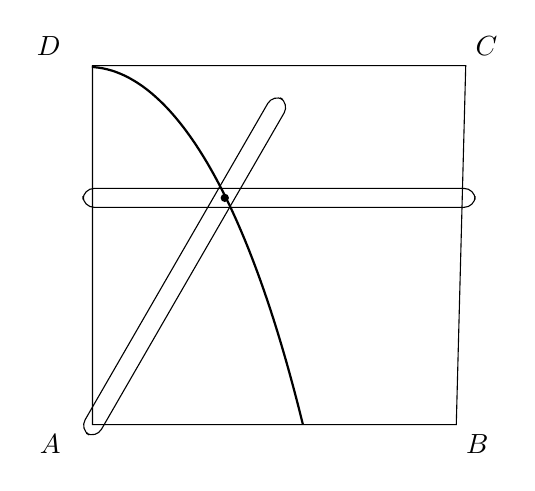
\begin{tikzpicture}[scale=.6,domain=.03:1.555,samples=100]
\draw (.1,.2) node[below left,xshift=-8pt] {$A$} -- (7.8,.2) node[below right] {$B$} -- (8,7.8) node[above right] {$C$} -- (.1,7.8) node[above left,xshift=-8pt] {$D$} -- cycle;
\draw[rounded corners,rotate=60] (0,-.2) rectangle (8.2,.2);
\draw[rounded corners] (-.1,4.8) rectangle (8.2,5.2);
\fill (2.9,5) circle [radius=2.5pt];
\draw[thick] plot (4.6*.637*\x,{12.2*.637*\x*cot(\x r)});
\end{tikzpicture}
\caption{Un compás de cuadraturiz}\label{f.trisect-quad-compass}
\end{center}
\end{minipage}
\end{figure}

Se puede construir una cuadratriz utilizando un compás de cuadratriz como se muestra en la figura~\ref{f.trisect-quad-compass}. Consiste en dos rectas (no marcadas) que se mueven como se ha descrito anteriormente. Una articulación las obliga a moverse simultáneamente y trazar la curva.
\begin{figure}[b]
\begin{center}
\begin{tikzpicture}[scale=.8,domain=.03:1.562,samples=100]
\draw (.1,7.8) coordinate (start)
  node[above left] {$D$}
  node[below right,xshift=32pt] {$\theta$} -- 
  (.1,.2) node[below left] {$A$} -- 
  (8,.1)  node[below right] {$B$} -- 
  (8,7.8) node[above right] {$C$} -- 
  cycle;
\draw[name path=curve,thick] plot (4.6*.637*\x,{12.2*.637*\x*cot(\x r)});
% To ensure intersection at node D, path should extend to the upper left of D
\coordinate (twenty-a) at ($(start)+(-35:9)$);
\path[name path=twenty] ($(start)!-.1!(twenty-a)$) -- (twenty-a);
\path[name path=sixty] (start) -- +(-50:11);
\path[name path=xaxis] (.1,.2) -- (8,.1);
\path[name intersections={of=twenty and curve,by={x1,tri}}];
\draw (start) -- (tri);
\node[above right] at (tri) {$P_2$};
\path[name intersections={of=sixty and curve,by={x2,angle}}];
\node[above right] at (angle) {$P_1$};
\draw (start) -- (angle);
\path[name intersections={of=xaxis and curve,by=x}];
\path[name intersections={of=sixty and xaxis,by=sixty-x}];
\draw (start) -- (sixty-x);

\path (tri) -- (tri -| .1,.2) coordinate (t3);
\draw[dashed] (t3) -- +(7.9,0);
\node[left] at (t3) {$F$};
\path (angle) -- (angle -| .1,.2) coordinate (t);
\draw[dashed] (t) -- +(7.9,0);
\node[left] at (t) {$E$};
\draw[<->] (-1.2,7.8) -- node[fill=white] {$t/3$} (-1.2,7.8 |- t3);
\draw[<->] (-.6,7.8) -- node[fill=white] {$t$} (-.6,7.8 |- t);
\draw[<->] (-.6,7.8 |- t) -- node[fill=white] {$1-t$} (-.6,.2);
\draw (3.5,7.8) arc[start angle=0,delta angle=-49,radius=3.5];
\draw (1,7.8) arc[start angle=0,delta angle=-32,radius=1];
\node at (3.3,6) {$\alpha$}; 
\end{tikzpicture}
\end{center}
\caption{Trisección de un ángulo mediante una cuadratriz}\label{f.trisect-quad-trisect}
\end{figure}

Se puede utilizar una cuadratriz para trisecar un ángulo.

\noindent\textbf{Construcción:}
Sea $\angle CDP_1=\alpha$ un ángulo arbitrario, donde $P_1$ es la intersección de la recta que define el ángulo $\alpha$ relativo a $\overline{DC}$ y la cuadratriz. Construyamos una recta que pase por $P_1$ paralela a $\overline{DC}$ y denotemos con $E$ su intersección con $\overline{AD}$. Denotemos $t$ el segmento $\overline{DE}$ por $t$ y trisequémoslo (Sec.~\ref{s.trisect-constructible}) para obtener el punto $F$ que está a $t/3$ de $\overline{DC}$. Sea $P_2$ la intersección de una recta desde $F$ paralela a $\overline{DC}$ y la cuadratriz, y denotemos por $\theta$ el ángulo entre $\overline{DC}$ y $\overline{DP_2}$ (Fig.~\ref{f.trisect-quad-trisect}).

\begin{theorem}
$\theta = \alpha/3$.
\end{theorem}
\begin{proof}
La coordenada $y$ de $E$ es $1-t$ por lo que por construcción la coordenada de $F$ es $y$ $1-(t/3)$. Puesto que la velocidad lineal constante de la línea horizontal es proporcional a la velocidad angular constante de la línea giratoria $\theta/\alpha = (t/3)/t$ y $\theta = \alpha/3$.
\end{proof}

%%%%%%%%%%%%%%%%%%%%%%%%%%%%%%%%%%%%%%%%%%%%%%%%%%%%%%%%%%%%%%%%%%

\section{Números construibles}\label{s.trisect-constructible}
\index{Constructible number}

Sea $l$ un segmento definido de longitud $1$.
\begin{definition}
Un número $a$ es \emph{constructible} si y sólo si se puede construir un segmento de longitud $a$ con regla y compás partiendo de $l$.
\end{definition}

Dado un segmento $l=\overline{AB}$, construir una recta que contenga a $\overline{AB}$ y utilizar el compás para encontrar un punto $C$ de la recta que esté a una distancia de $1$ de $B$. Entonces $\overline{AC}$ tiene una longitud $2$ por lo que el número $2$ es construible. Se puede construir un segmento $\overline{BD}$ de longitud $1$ perpendicular a $\overline{AB}$ en $B$. La hipotenusa del triángulo $\triangle ABD$ es de longitud $\sqrt{2}$ por lo que el número $\sqrt{2}$ es construible.

\begin{theorem}\label{thm.trisect-constructible}
Un número es \emph{construible} si y sólo si es el valor de una expresión construida a partir de los números enteros, las cuatro operaciones aritméticas $\{+,-,\times,/\}$ y la operación de sacar raíz cuadrada $\surd$.
\end{theorem}

\begin{proof} Primero demostramos que los valores de estas expresiones son construibles.
\index{Constructible number!arithmetic operation}

\begin{figure}[b]
\begin{center}
\begin{tikzpicture}[scale=.8]
\coordinate (P) at (0,0);
\coordinate (Q) at (5,0);
\coordinate (T) at (3,0);
\coordinate (U) at (7,0);
\vertex{P};
\vertex{Q};
\draw (P) -- (Q);
\node[above] at (P) {$P$};
\node[above left] at (Q) {$Q$};
\node[above left] at (U) {$U$};
\node[above right] at (T) {$T$};
\draw (5,0) -- (8,0);
\draw (5,0) circle[radius=2cm];
\draw (5,0) -- node[left] {$b$} ++(60:2cm);
\coordinate (R) at (9,-1);
\coordinate (S) at ($(9,-1) + (20:2cm)$);
\vertex{R};
\vertex{S};
\draw (R) node[above] {$R$} --
  node[below right] {$b$} (S)
  node[above] {$S$};
\draw[<->] (0,-.5) -- node[fill=white] {$a$} (5,-.5);
\draw[<->] (0,-1) -- node[fill=white] {$a-b$} (3,-1);
\draw[<->] (0,-1.5) -- node[fill=white] {$a+b$} (7,-1.5);
\end{tikzpicture}
\end{center}
\caption{Construcción de sumas y restas}\label{f.trisect-add-subtract}
\end{figure}

\noindent\textbf{Suma y resta:}
Dados los segmentos $\overline{PQ}=a$ y $\overline{RS}=b$, construir una circunferencia centrada en $Q$ con radio $b$ (Fig.~\ref{f.trisect-add-subtract}). Extender $\overline{PQ}$ hasta que se cruza con la circunferencia en $U$. Entonces $\overline{PTQU}$ es un segmento, donde $\overline{PT}=a-b$ y $\overline{PU}=a+b$.

\noindent\textbf{Multiplicación:}
Por triángulos similares en la figura~\ref{f.trisect-multiplication},
$(1/b)=(a/\overline{OA})$, así que $\overline{OA}=ab$.

\noindent\textbf{División:}
Por triángulos similares en la figura~\ref{f.trisect-division},
$(1/b)=(\overline{OD}/a)$, así que $\overline{OD}=(a/b)$.

\begin{figure}[t]
\begin{minipage}{.48\textwidth}
\begin{center}
\begin{tikzpicture}[scale=.8]
\draw[name path=horz] (0,0) coordinate (o) -- (7,0);
\node[left] at (o) {$O$};
\coordinate (a) at (6,0);
\node[below]  at (a) {$A$};
\draw (o) -- (30:5.5);
\coordinate (c) at (30:3);
\coordinate (b) at (30:5);
\node[above] at (c) {$C$};
\node[above] at (b) {$B$};
\draw (a) -- (b);
\path[name path=par] (c) -- +($(a)-(b)$);
\path[name intersections={of=par and horz,by=d}];
\node[below] at (d) {$D$};
\draw (c) -- (d);
\draw[<->] (-.4,.5) -- node[fill=white] {$b$} +(30:5.2);
\path (o) -- node[above] {$1$} (c);
\draw[<->] (0,-.8) -- node[fill=white] {$ab$} +(6,0);
\path (o) -- node[below] {$a$} (d);
\end{tikzpicture}
\caption{Construcción de la multiplicación}\label{f.trisect-multiplication}
\end{center}
\end{minipage}
\hfill
\begin{minipage}{.48\textwidth}
\begin{center}
\begin{tikzpicture}[scale=.8]
\draw[name path=horz] (0,0) coordinate (o) -- (7,0);
\node[left] at (o) {$O$};
\coordinate (a) at (6,0);
\node[below]  at (a) {$A$};
\draw (o) -- (30:5.5);
\coordinate (c) at (30:3);
\coordinate (b) at (30:5);
\node[above] at (c) {$C$};
\node[above] at (b) {$B$};
\draw (a) -- (b);
\path[name path=par] (c) -- +($(a)-(b)$);
\path[name intersections={of=par and horz,by=d}];
\node[below] at (d) {$D$};
\draw (c) -- (d);
\draw[<->] (-.4,.5) -- node[fill=white] {$b$} +(30:5.2);
\path (o) -- node[above] {$1$} (c);
\draw[<->] (0,-.8) -- node[fill=white] {$a$} +(6,0);
\path (o) -- node[below] {$a/b$} (d);
\end{tikzpicture}
\caption{Construcción de la división}\label{f.trisect-division}
\end{center}
\end{minipage}
\end{figure}

\noindent\textbf{Raíces cuadradas:}
Dado un segmento $\overline{BC}=a$, construyamos $\overline{AB} =1+a$ y una semicircunferencia con $\overline{AB}$ como diámetro. Construyamos una perpendicular en $C$ y sea $D$ la intersección de la perpendicular y la circunferencia (Fig.~\ref{f.trisect-square-root}). El $\angle ADB$ es un ángulo recto porque está subtendido por un diámetro. Por triángulos semejantes $(h/1)=(a/h)$, por lo que $h^2=a$ y $h=\sqrt{a}$.

\begin{figure}[b]
\begin{center}
\begin{tikzpicture}[scale=1]
\draw[name path=horz] (0,0) coordinate (a) -- (6,0);
\node[left] at (a) {$A$};
\coordinate (b) at (6,0);
\node[below] at (b) {$B$};
\draw[name path=circle] (b) arc(0:180:3);
\path[name path=perp] (2,0) -- +(0,3.2);
\coordinate (c) at (2,0);
\node[below] at (c) {$C$};
\path[name intersections={of=circle and perp,by=d}];
\node[above] at (d) {$D$};
\draw (c) -- node[right] {$h$} (d);
\path (a) -- node[below] {$1$} (c) -- node[below] {$a$} (b);
\draw (c) rectangle +(6pt,6pt);
\draw (a) -- (d) -- (b);
\draw[rotate=-125] (d) rectangle +(6pt,6pt);
\node[above right,xshift=4pt] at (a) {$\alpha$};
\node[above left,xshift=-12pt] at (b) {$90^\circ\!-\!\alpha$};
\node[below right,yshift=-8pt] at (d) {$\alpha$};
\node[below left,xshift=0pt,yshift=-18pt] at (d) {$90^\circ\!-\!\alpha$};
\end{tikzpicture}
\end{center}
\caption{Construcción de una raíz cuadrada}
\label{f.trisect-square-root}
\end{figure}

Para demostrar la inversa del teorema, necesitamos determinar qué expresiones se pueden construir con una regla y un compás. Hay tres construcciones\footnote{Para mayor claridad se ilustran para valores específicos en lugar de las ecuaciones más generales.}:

\begin{enumerate}
\item Dos rectas se intersecan en un punto (Fig.~\ref{f.constructible-two-lines}). Las coordenadas de la intersección pueden deducirse de las ecuaciones de las dos rectas $y=x$ y $y=4x-2$. El punto de intersección es $P= (2/3, 2/3)$.

\item Una recta interseca a una circunferencia en cero, uno o dos puntos (Fig.~\ref{f.constructible-line-circle}). Las coordenadas de las intersecciones pueden deducirse de las ecuaciones de la recta $y=x$ y la circunferencia $x^2+y^2=4$. Los puntos de intersección son
$P=(\sqrt{2}, \sqrt{2})$ y $Q=(-\sqrt{2}, -\sqrt{2})$.

\item Dos circunferencias se intersecan en cero, uno o dos puntos (Fig.~\ref{f.constructible-two-circles}). Las coordenadas de las intersecciones pueden deducirse de las ecuaciones de las dos circunferencias $(x-1)^2+y^2=4$, $(x+1)^2+y^2=4$. Los puntos de intersección son $P=(0,\sqrt{2}),Q=(0,-\sqrt{2})$.
\end{enumerate}
\end{proof}

\begin{figure}[t]
\begin{minipage}{.45\textwidth}
\begin{tikzpicture}[scale=.66]
\draw[step=10mm,white!50!black,very thin] (-4,-4) grid (4,4);
\draw[thick] (-4,0) -- (4,0);
\draw[thick] (0,-4) -- (0,4);
\coordinate (O) at (0,0);
\foreach \x in {-3,...,4}
  \node at (\x-.2,-.3) {\sm{\x}};
\foreach \y in {-3,...,-1}
  \node at (-.4,\y-.3) {\sm{\y}};
\foreach \y in {1,...,4}
  \node at (-.3,\y-.3) {\sm{\y}};
\draw[name path=eq1] (-4,-4) -- (4,4);
\draw[name path=eq2] (-.5,-4) -- (1.5,4);
\path[name intersections={of=eq1 and eq2,by={P}}];
\node[right] at (P) {$P$};
\end{tikzpicture}
\caption{El punto de intersección de dos líneas}\label{f.constructible-two-lines}
\end{minipage}
\hfill
\begin{minipage}{.45\textwidth}
\begin{tikzpicture}[scale=.66]
\coordinate (O) at (0,0);
\draw[step=10mm,white!50!black,very thin] (-4,-4) grid (4,4);
\draw[thick] (-4,0) -- (4,0);
\draw[thick] (0,-4) -- (0,4);
\foreach \x in {-3,...,4}
  \node at (\x-.2,-.3) {\sm{\x}};
\foreach \y in {-3,...,-1}
  \node at (-.4,\y-.3) {\sm{\y}};
\foreach \y in {1,...,4}
  \node at (-.3,\y-.3) {\sm{\y}};
\coordinate (A) at (2,0);
\node[draw,circle through=(A),name path=circle] at (0,0) {};
\draw[name path=eq1] (-4,-4) -- (4,4);
\path[name intersections={of=eq1 and circle,by={P,Q}}];
\node[right] at (P) {$P$};
\node[left] at (Q) {$Q$};
\end{tikzpicture}
\caption{Los puntos de intersección de una recta y una circunferencia}\label{f.constructible-line-circle}
\end{minipage}
\end{figure}

\begin{figure}[b]
\begin{center}
\begin{tikzpicture}[scale=.66]
\coordinate (O) at (0,0);
\draw[step=10mm,white!50!black,very thin] (-4,-4) grid (4,4);
\draw[thick] (-4,0) -- (4,0);
\draw[thick] (0,-4) -- (0,4);
\foreach \x in {-3,...,4}
  \node at (\x-.2,-.3) {\sm{\x}};
\foreach \y in {-3,...,-1}
  \node at (-.4,\y-.3) {\sm{\y}};
\foreach \y in {1,...,4}
  \node at (-.3,\y-.3) {\sm{\y}};
\coordinate (A) at (3,0);
\node[draw,circle through=(A),name path=circle1] at (1,0) {};
\coordinate (B) at (-3,0);
\node[draw,circle through=(B),name path=circle2] at (-1,0) {};
\path[name intersections={of=circle1 and circle2,by={P,Q}}];
\node[right,xshift=6pt,yshift=-2pt] at (P) {$P$};
\node[right,xshift=6pt,yshift=2pt] at (Q) {$Q$};
\end{tikzpicture}
\caption{Los puntos de intersección de dos círculos}\label{f.constructible-two-circles}
\end{center}
\end{figure}

%%%%%%%%%%%%%%%%%%%%%%%%%%%%%%%%%%%%%%%%%%%%%%%%%%%%%%%%%%%%%%%%%

\section{Números construibles como raíces de polinomios}\label{s.trisect-poly}

Para demostrar que un número no es construible, tenemos que demostrar que no se puede expresar utilizando sólo números enteros y las operaciones $ {+,-,\times,/,\surd}$.

Demostraremos que los números construibles son las raíces de una cierta clase de polinomios y luego demostraremos que la trisección de un ángulo y la duplicación de un cubo requieren la construcción de raíces de polinomios que no están en esta clase. Hoy en día estos resultados se demuestran utilizando la teoría de campos del álgebra abstracta, pero aquí doy una demostración que utiliza matemáticas elementales. La demostración se basa en la siguiente definición.

\begin{definition}
El \emph{profundidad} de una expresión construida a partir de los enteros y los operadores $\{+,-,\times,/,\surd\}$ es el máximo nivel de anidamiento de raíces cuadradas.
\end{definition}\index{Constructible number!depth of square roots}

\begin{example}
Consideremos la siguiente expresión:
\[
\sqrt{17+3\sqrt{17} - \sqrt{34-2\sqrt{17}}
  -2\sqrt{34+2\sqrt{17}} }\,.
\]
La profundidad es $3$ porque a la derecha de la expresión tenemos $\sqrt{17}$ que está anidado dentro de $\sqrt{34+2\sqrt{17}}$, que a su vez está anidado dentro de:
\[
\sqrt{17+\cdots-\cdots-2\sqrt{34+2\sqrt{17}}}\,.
\]
\end{example}

\begin{theorem}
Una expresión de profundidad $n$ puede expresarse como $a+b\sqrt{c}$ donde $a,b,c$ son expresiones de profundidad como máximo $n-1$.
\end{theorem}
\begin{proof}
Cálculos sencillos muestran que las expresiones $(a_1+b_1\sqrt{c}),\mathit{op}\,(a_2+b_2\sqrt{c})$ para los operadores $\mathit{op}=\{+,-,\times\}$ resultan en expresiones $a+b\sqrt{c}$ de profundidad $n-1$. Para la división el cálculo es un poco más complicado:
\begin{eqnarray*}
\frac{a_1+b_1\sqrt{c}}{a_2+b_2\sqrt{c}}&=&
\frac{(a_1+b_1\sqrt{c})(a_2-b_2\sqrt{c_2})}{(a_2+b_2\sqrt{c})(a_2-b_2\sqrt{c})}\\
&=&\frac{a_1a_2-b_1b_2c}{a_2^2-b_2^2c}+\frac{a_2b_1-a_1b_2}{a_2^2-b_2^2c}\sqrt{c}\,,
\end{eqnarray*}
que es de la forma $a+b\sqrt{c}$ donde $a,b,c$ son de profundidad $n-1$.
Por último, la raíz cuadrada de una expresión de profundidad $n-1$ es una expresión de profundidad $n$.
\end{proof}

\begin{theorem}\label{thm.trisect.conjugate}
Sea $p(x)$ un polinomio cúbico mónico con coeficientes racionales:
\[
p(x)=x^3+a_2x^2+a_1x+a_0\,,
\]
y sea $r=a+b\sqrt{c}$ una raíz de $p(x)$ \emph{de profundidad mínima} $n$, donde $a,b,c$ son de profundidad (como máximo) $n-1$. Entonces $r'=a-b\sqrt{c}$ es una raíz de $p(x)$ y $r\neq r'$.
\end{theorem}\index{Roots!cubic@of cubic polynomials|(}

\begin{proof}
Calculemos $p(r)$ que es igual a $0$ ya que $r$ es una raíz:
\[
\renewcommand{\arraystretch}{1.4}
\begin{array}{lcr}
(a+b\sqrt{c})^3+a_2(a+b\sqrt{c})^2+a_1(a+b\sqrt{c})+a_0&=\\
(a^3+3a^2b\sqrt{c}+3ab^2c+b^3c\sqrt{c})\\
\quad+\,a_2(a^2+2ab\sqrt{c}+b^2c) +a_1(a+b\sqrt{c}) +a_0&=\\
(a^3+3ab^2c+a_2a^2+a_2b^2c+a_1a+a_0)\\
\quad+\,(3a^2b+b^3c+2a_2ab+a_1b)\sqrt{c}&=\\
d+e\sqrt{c}&=&0\,.
\end{array}
\]
donde $d,e$ son expresiones de profundidad $n-1$ formadas a partir de los coeficientes racionales y $a,b,c$. Entonces $\sqrt{c}=-d/e$, por lo que $a+b\sqrt{c}$ se puede expresar como una expresión de profundidad $n-1$, contradiciendo la suposición de que $a+b\sqrt{c}$ es de profundidad mínima $n$. Como $\sqrt{c}\neq 0$ y es de profundidad $n$, para que $d+e\sqrt{c}$ sea cero debe ser que $d=e=0$.

Consideremos ahora $r'=a-b\sqrt{c}$. Examinando el cálculo anterior vemos que $p(r')=d-e\sqrt{c}=0+0\cdot\sqrt{c}=0$, por lo que $r'$ también es una raíz de $p$.

Si $r= r'$ entonces $0=r-r'=2b\sqrt{c}$, lo cual es cierto sólo si $b=0$ por lo que $r,r'$ sería de profundidad $n-1$, contradiciendo de nuevo la suposición.
\end{proof}                                

\begin{theorem}
Si un polinomio mónico cúbico con coeficientes racionales:
\[p(x)=x^3+a_2x^2+a_1x+a_0\] no tiene raíces racionales entonces ninguna de sus raíces es construible.
\end{theorem}

\begin{proof}
Por el Teorema Fundamental del Álgebra  (Teorema~\ref{thm.fundamental}) $p(x)$ tiene tres raíces $r_1,r_2,r_3$. Sea $r_1=a+b\sqrt{c}$ una raíz de profundidad mínima $n$. Por la suposición de que no hay raíces racionales, $n\geq 1$, y por tanto $b\neq 0$ y $c\neq 0$. Por Teorema~\ref{thm.trisect.conjugate}, $r_2=a-b\sqrt{c}$ también es una raíz. Realicemos la siguiente multiplicación:
\begin{subeqnarray}
(x-r_1)(x-r_2)(x-r_3)&=&x^3 -(r_1+r_2+r_3)x^2\\
&&\quad\; +\, (r_1r_2+r_1r_3+r_2r_3)x + r_1r_2r_3\slabel{eq.viete3}\\
a_2&=&-(r_1+r_2+r_3)\\
r_3&=&-(a_2+r_1+r_2)\,.
\end{subeqnarray}
Como $a_2$ es racional también lo es:
\[r_3=-a_2-(r_1+r_2)=-a_2-2a\,,\]
contradiciendo la suposición.
\end{proof}
\index{Roots!cubic@of cubic polynomials|)}

%%%%%%%%%%%%%%%%%%%%%%%%%%%%%%%%%%%%%%%%%%%%%%%%%%%%%

\section{Imposibilidad de las Construcciones Clásicas}\label{s.trisect-impossible}

\begin{theorem}\label{thm.trisect.cube-root-irrational}
$\sqrt[3]{2}$ es irracional.
\end{theorem}
\begin{proof}
Supongamos que $\sqrt[3]{2}$ es racional e igual a $p/q$ donde $p,q$ son enteros sin factores comunes distintos de $\pm 1$. Entonces:
\begin{eqnarray*}
(p/q)^3&=&(\sqrt[3]{2})^3\\
p^3&=&2q^3\,,
\end{eqnarray*}
por lo que $p$ debe ser divisible por $2$, digamos $p=2r$. Ahora:
\begin{eqnarray*}
8r^3&=&2q^3\\
q^3&=&4r^3\,,
\end{eqnarray*}
por lo que $q$ es divisible por $2$, contradiciendo la suposición de que $p,q$ no tienen factor común.
\end{proof}

\begin{theorem}
$x^3-2$ no tiene raíces racionales por lo que es imposible duplicar el volumen de un cubo con una regla y un compás.
\end{theorem}
\begin{proof}
Una de sus raíces es $\sqrt[3]{2}$ que por Teorema~\ref{thm.trisect.cube-root-irrational} es irracional. Las otras raíces son las raíces de la ecuación cuadrática $x^2+\sqrt[3]{2}x+(\sqrt[3]{2})^2$ que se obtiene dividiendo $x^3-2$ entre $x-\sqrt[3]{2}$. Es fácil comprobar que sus raíces no son racionales (de hecho, ni siquiera reales).
\end{proof}

\begin{theorem}
Es imposible trisecar un ángulo arbitrario con una regla y un compás.
\end{theorem}
\begin{proof}
Basta con demostrar la imposibilidad para un ángulo. Intentemos trisecar $60^\circ$ para obtener $20^\circ$. Por el Teorema~\ref{thm.triple-angle}:
\begin{eqnarray*}
\cos 3\alpha&=&4\cos^3\alpha -3\cos\alpha\\
\cos 60^\circ&=&4\cos^3 20^\circ -3\cos 20^\circ\,.
\end{eqnarray*}
Denotemos $x=\cos 20^\circ$ y $2x$ por $y$. Como $\cos 60^\circ=1/2$ tenemos:
\begin{eqnarray*}
4x^3 -3x-\frac{1}{2} &=& 0\\
8x^3-6x-1&=&0\\
y^3-3y-1&=&0\,.
\end{eqnarray*}

Para demostrar que el polinomio $y^3-3y-1$ no tiene raíces racionales supongamos que $y=a/b$ es una raíz racional con $a,b$ que no tienen ningún factor común distinto de $\pm 1$. Entonces:
\begin{subeqnarray}
(a/b)^3-3(a/b)-1&=&0\\
a^3-3ab^2&=&b^3\\
a(a-3b^2)&=&b^3\slabel{eq.trisect1}\\
a^3&=&b(b^2+3ab)\slabel{eq.trisect2}\,.
\end{subeqnarray}
Por la ecuación~\ref{eq.trisect1}, $b$ debe ser divisible por $a$, y por la ecuación~\ref{eq.trisect2}, $a$ debe ser divisible por $b$, lo que sólo es posible si $a=b=\pm 1$ y $a/b=\pm 1$. Por cálculo, $y=a/b=1$ y $y=a/b=-1$ no son raíces del polinomio.
\end{proof}

Una forma alternativa de demostrar la imposibilidad de las construcciones es utilizar el siguiente teorema que presentamos sin demostración.

\begin{theorem}\label{thm.factor}
Si un polinomio mónico $p(x)=x^n+a_{n-1}x^{n-1}+\cdots+a_0$ con coeficientes enteros tiene raíces racionales entonces tiene raíces enteras.
\end{theorem}

Para demostrar la imposibilidad de duplicar un cubo necesitamos demostrar que:
\[
x^3-2=(x-r_2)(x-r_1)(x-r_0)
\]
no tiene raíces enteras. Como $r_0r_1r_2=-2$, todas las raíces deben dividir a $2$, así que las únicas raíces enteras posibles son $\pm 1, \pm 2$. Un cálculo rápido muestra que ninguna de ellas es raíz.

Para demostrar la imposibilidad de trisecar un ángulo hay que demostrar que $y^3-3y-1$ no tiene raíces enteras. Una raíz entera debe dividir a $-1$ pero ni $1$ ni $-1$ son raíces.

\subsection*{¿Cuál es la sorpresa?}

Underwood Dudley ha realizado un extenso estudio de lo que él llama <<gruñones>>, que malgastan años de sus vidas intentando trisecar ángulos con una regla y un compás. No sólo se engañan a sí mismos pensando que esto es posible, sino que, lo que es peor, piensan que una solución sería importante. Por supuesto, una solución no tendría ninguna utilidad práctica, ya que herramientas como el neusis y la cuadratriz pueden resolver el problema con exactitud. El número de construcciones de este tipo es sorprendente, sobre todo porque muchas de ellas son ingeniosas y consiguen buenas aproximaciones. Calcular las fórmulas asociadas a las construcciones es un excelente ejercicio de trigonometría.

También es sorprendente que las demostraciones de la imposibilidad de estas construcciones geométricas sean puramente algebraicas, utilizando propiedades de raíces de polinomios.

\subsection*{Fuentes}

Wikipedia \cite{wiki:tri, wiki:neu, wiki:quad} es una buena fuente para las construcciones de este capítulo. Las dos trisecciones aproximadas proceden de \cite[pp.~67--68, 95--96]{dudley-budget}. El segundo ejemplo se atribuye al famoso filósofo Thomas Hobbes. Tanto \cite[pp.~48--49]{martin} como \cite[pp.~6--7]{dudley-budget} discuten la trisección usando la cuadratriz.
La duplicación del cubo usando un neusis está tomada de \cite{dorrie2}.

Un tratamiento riguroso de la constructibilidad se puede encontrar en los libros de texto sobre álgebra abstracta como \cite{fraleigh}, que contiene una demostración general de la inversa de Teorema~\ref{thm.trisect-constructible} en Sec.~32. Teorema~\ref{thm.factor} es Teorema~23.11 de \cite{fraleigh}. Una presentación relativamente accesible de la demostración de Wantzel se puede encontrar en \cite{suzuki}. Mi presentación de la constructibilidad se basa en las presentaciones en \cite[Capítulo~III]{courant} y \cite{laugwitz}.
